\begin{appendices}

%Some Table of Contents entry formatting
\addtocontents{toc}{\protect\renewcommand{\protect\cftchappresnum}{\appendixname\space}}
\addtocontents{toc}{\protect\renewcommand{\protect\cftchapnumwidth}{6em}}

%Begin individual appendices, separated as chapters

\chapter[\texorpdfstring{Linklet Kernel Language Specification}{Appendix A}]{Linklet Kernel Language Specification}
\label{appendix:linklet-kernel-language}

    \inputAppendixFigure{linklet-kernel-language-grammar.tex}

    \begin{figure}[h]
    \centering
    \fbox{
        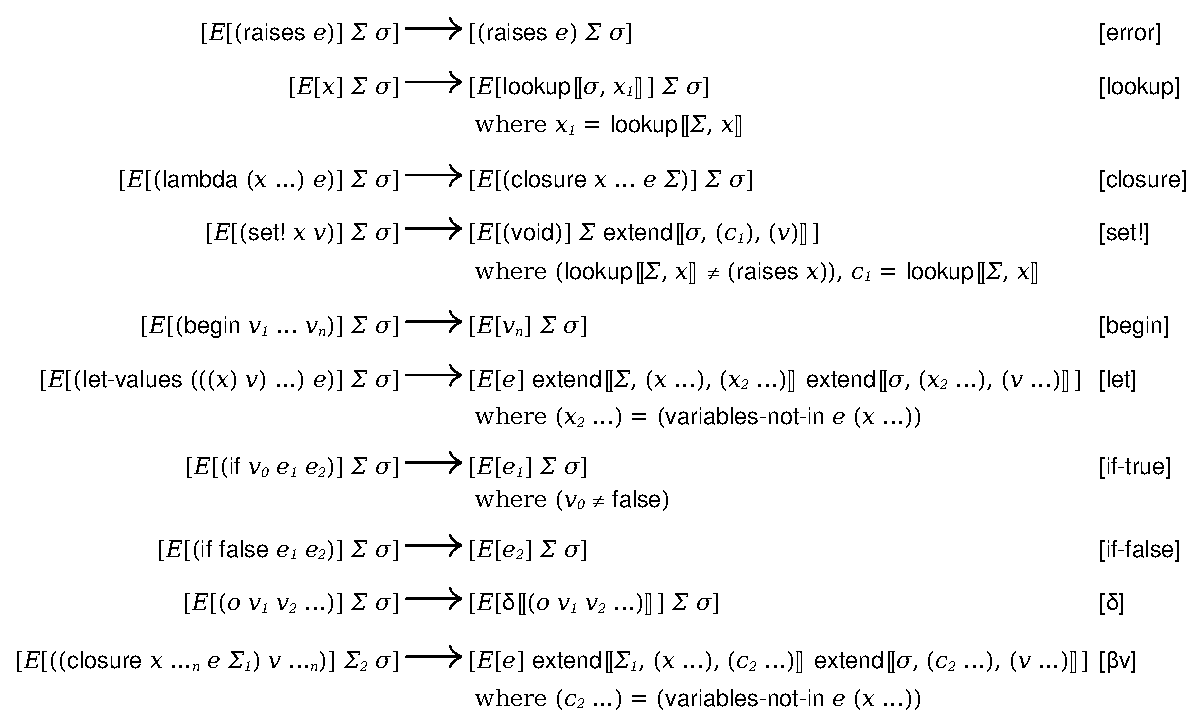
\includegraphics[scale=0.8]{sections/figures/rc-red-relation.eps}
    }
    \caption{Linklet Kernel Language standard reduction relation}
    \label{fig:rc-red-relation}
    \end{figure}

    \begin{figure}[h]
    \centering
    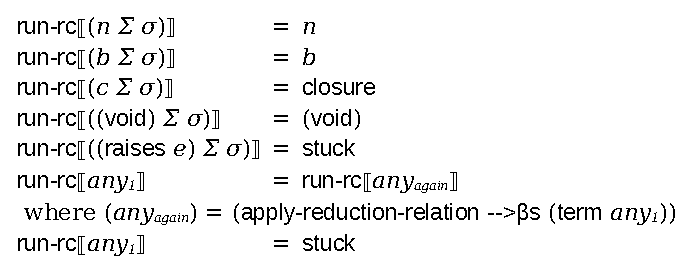
\includegraphics[scale=1]{sections/figures/rc-run-rc.eps}
    \caption{Linklet Kernel Language evaluator}
    \label{fig:rc-run-rc}
    \end{figure}


\chapter[\texorpdfstring{Complete Reduction Steps for Top-level Example Program}{Appendix B}]{Complete Reduction Steps for Top-level Example Program}
\label{appendix:formal-reduction-steps-toplevel-example}

    \inputAppendixFigure{complete-toplevel-example-step-by-step-formal.tex}

\chapter[\texorpdfstring{PLT Redex Model for Linklet Semantics}{Appendix C}]{PLT Redex Model for Linklet Semantics}
\label{appendix:linklet-semantics-model-redex-code}

    \inputAppendixFigure{linklet-semantics-plt-redex-model.tex}

\chapter[\texorpdfstring{Semantics for the CEK \& Stackful Hybrid Model}
                          {Appendix D}]{Semantics for the CEK \& Stackful Hybrid Model}
\label{appendix:cek-stackful-redex}

    \begin{figure}[!htbp]
    \centering
    \begin{align*}
        e &::=\; x \;|\; v \;|\; (e\; e\;\ldots) \;|\; (\textbf{if}\; e\; e\; e) \;|\; (\textit{op}\; e\;\ldots)\\
          &\;\hspace*{1.5em}|\; (\textbf{set!}\; x\; e) \;|\; (\textbf{begin}\; e\; e\;\ldots) \;|\; (\textbf{lambda}\; (x_{\_}\;\ldots)\; e)\\
          &\;\hspace*{1.5em}|\; (\textbf{let-values}\; (((x_{\_})\; e)\;\ldots)\; e) \;|\; (\textbf{letrec-values}\; (((x_{\_})\; e)\;\ldots)\; e)\\
          &\;\hspace*{1.5em}|\; \mathit{internal\text{-}letrec} \;|\; (\textbf{raises}\; e) \;|\; (\textbf{raise-depth}) \;|\; (\textbf{convert-stack}\; e)\\
          &\;\hspace*{1.5em}|\; \mathit{convert} \;|\; \mathit{stuck}\\[0.3em]
        v &::=\; n \;|\; b \;|\; c \;|\; (\textbf{void})\\
        c &::=\; (\textbf{closure}\; x\;\ldots\; e\; \rho)\\
        n &::=\; \textit{number}\\
        b &::=\; \textbf{true} \;|\; \textbf{false}\\
        x,\; \textit{cell} &::=\; \textit{variable-not-otherwise-mentioned}\\
        op &::=\; \textbf{add1} \;|\; + \;|\; * \;|\; < \;|\; \textbf{sub1}\\
        \rho &::=\; ((x\; \textit{any})\;\ldots)\\
        \Sigma &::=\; ((x\; \textit{any})\;\ldots)\\[0.3em]
        \mathit{internal\text{-}letrec} &::=\; (\textbf{letrec-values-cell-ready}\; (((x_{\_})\; e)\;\ldots)\; e)\\
        \mathit{convert} &::=\; (\textbf{convert-to-stackful}\; e) \;|\; (\textbf{convert-to-cek}\; e)\\
                        &\;\hspace*{1.5em}|\; (\textbf{convert-stack-to-heap}\; \rho\; \Sigma\; x)\\
        \mathit{exception} &::=\; (\textbf{stack-depth-exn}\; n) \;|\; (\textbf{convert-to-cek-exn}\; e\; \rho\; \Sigma)\\
        \mathit{rc\text{-}result} &::=\; v \;|\; \mathit{stuck}\\[0.3em]
        \kappa &::=\; (x\;\ldots)\\
               &\;|\; (\textbf{if-}\kappa\; e\; e)\\
               &\;|\; (\textbf{arg-}\kappa\; (e\;\ldots))\\
               &\;|\; (\textbf{fun-}\kappa\; c\; (e\;\ldots)\; (v\;\ldots))\\
               &\;|\; (\textbf{set-}\kappa\; x)\\
               &\;|\; (\textbf{seq-}\kappa\; e\;\ldots)\\
               &\;|\; (\textbf{op-}\kappa\; \textit{op}\; (v\;\ldots)\; (e\;\ldots)\; \rho)\\
               &\;|\; (\textbf{let-}\kappa\; (((x)\; e)\;\ldots)\; (x\;\ldots)\; (v\;\ldots)\; e)\\
               &\;|\; (\textbf{letrec-}\kappa\; (((x)\; e)\;\ldots)\; x\; e)
    \end{align*}

    \vspace{-1em}

    \caption{Source Language for Stackful \& CEK Model}
    \label{fig:st-cek-grammar}
\end{figure}

    \clearpage

    \inputAppendixFigure{cek-reduction-relation-redacted-general}

    \inputAppendixFigure{cek-reduction-relation-redacted-letrec}

    \inputAppendixFigure{cek-reduction-relation-redacted-application}

    \clearpage

    \inputAppendixFigure{stackful-semantics.tex}

\end{appendices}